\clearpage
\subsubsection{MSVC + \olly}
\index{\olly}

\RU{Загрузим пример в}\EN{Let's load our example into} \olly 
\RU{и увидим, какие значения были установлены в EAX/EBX/ECX/EDX после
исполнения}\EN{and see, what values are set in EAX/EBX/ECX/EDX after the execution of} CPUID: 

\begin{figure}[H]
\centering
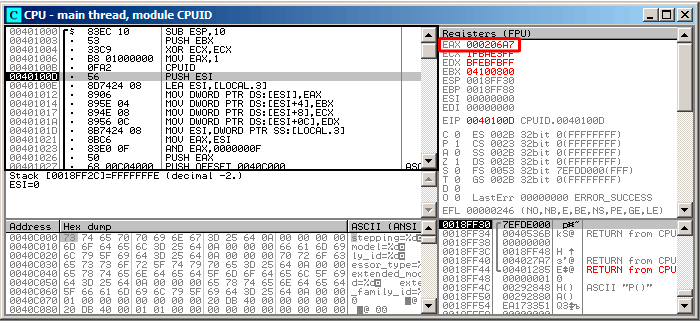
\includegraphics[scale=\FigScale]{patterns/15_structs/6_bitfields/cpuid/olly.png}
\caption{\olly: \RU{После исполнения CPUID}\EN{After CPUID execution}}
\label{fig:cpuid_olly_1}
\end{figure}

\RU{В EAX установлено}\EN{EAX has} \TT{0x000206A7} 
(\RU{мой}\EN{my} \ac{CPU} \EN{is}\RU{---} Intel Xeon E3-1220).\\
\RU{В двоичном виде это}\EN{This is} $0000 0000 0000 0010 0000 0110 1010 0111$\EN{ in binary form}.

\RU{Вот как распределяются биты по полям в моем случае}\EN{Here is how the bits are distributed by fields}:

\begin{center}
\begin{tabular}{ | l | l | l | }
\hline
\headercolor{} \RU{поле}\EN{field} &
\headercolor{} \RU{в двоичном виде}\EN{in binary form} &
\headercolor{} \RU{в десятичном виде}\EN{in decimal form} \\
\hline
reserved2		& 0000 & 0 \\
\hline
extended\_family\_id	& 00000000 & 0 \\
\hline
extended\_model\_id	& 0010 & 2 \\
\hline
reserved1		& 00 & 0 \\
\hline
processor\_id		& 00 & 0 \\
\hline
family\_id		& 0110 & 6 \\
\hline
model			& 1010 & 10 \\
\hline
stepping		& 0111 & 7 \\
\hline
\end{tabular}
\end{center}

\begin{figure}[H]
\centering
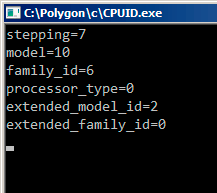
\includegraphics[scale=\NormalScale]{patterns/15_structs/6_bitfields/cpuid/result.png}
\caption{\olly: \RU{Результат работы}\EN{Result}}
\label{fig:cpuid_olly_2}
\end{figure}
